\section{Proposed Technical Work}

To help support testing my hypotheses, a number of new pieces of technology and instruction will need to be created.

\subsection{Normalization of Difficulty}

Programming knowledge

Domain knowledge

\subsection{Instructor Guides}

\subsection{Developer Guides}

\subsection{Data Discoverability}

Understanding the structure, meaning, and values of data can be a difficult problem for introductory students.
Using Data Science as the introductory context puts an increased emphasis on data structures and algorithms, making this content more critical for the learner.
Currently, there are not many tools available through Kennel to scaffold students.

The Property Explorer is probably the current greatest tool available to students for understanding program state.
However, field trials with it show that most students do not take advantage of the tool, with few reported events in the systems' tracker.
The usability of the property explorer, and its connection to the concept of Program State, must be elucidated to the student more clearly.

More tools are also desirable for engaging learners.
A number of graphical representations are used throughout the Computational Thinking course in order to visualize topics such as Abstraction and program flow.
For instance, students build Data Map Diagrams as seen in Figure \ref{data-maps-weather}, intended to help them navigate complex data structures.
The system can be extended to create simplified graphical visualizations of the students code and the data model in order to connect to these other course topics.

Currently, the implementation of MatPlotLib and other APIs is very minimal -- eventually, complete support for their functionality is needed.
There are other novel additions that can be introduced too -- for example, recent work by \cite{pixly} integrates media computation into Blockly environments.
By integrating such material into Kennel, we can provide students a comparative point between the different introductory programming contexts, in order to meaningfully evaluate the affordances of the different approaches.
Crucially, care must be taken to keep Kennel as a pure Python programming environment, without introducing cumbersome non-standard 3rd party libraries as occurs in CodeSkulptor~\cite{code-skulptor}.
As all of these materials extend the functionality of Kennel is new and innovating ways, but this material is less valuable if it reduces the authenticity and transferability of the learning experience.

\subsection{More Libraries}

The CORGIS project depends on having an extensive and varied collection of datasets. 
Students should be able to find a dataset that appeals to their personal interests but provides a sound learning experience.
Making this experience relatively uniform is challenging, but makes providing support much easier -- a necessary element in a scaled classroom.

The same data source can be expressed in many ways, representing different levels of abstraction and different affordances.
Consider the data map in figure \ref{data-maps-weather}, representing potential structures for weather data collected about cities around the world.
Although maps A and B contain the exact same data, they are structured very differently -- a list of cities vs. a dictionary of cities.
For an experienced programmer, these differences are minor details that have implications for runtime performance: looking up a city's temperature is slower and more complicated in structure A (requring iteration and decision) than it is in B (requiring only dictionary access).
Although the differences in code are minor to an expert, they require fundamentally different areas of knowledge for a beginner.
Map C represents an entirely different level of abstraction, where weather is only represented as a numeric, without information about cities.
The number of questions that can be answered using this data is greatly reduced -- statistics about cities in general, rather than comparisons against specific cities.
And of course, the nature and schema of the data itself affects the types of questions that can be asked -- it makes sense to find the average of a list of temperatures, but not the sum.
A key part of my research will be explicitly identifies trade-offs and affordances of different structures and abstractions of data.

\begin{figure}
\begin{center}
\tikzset{
    bnode/.style = {   
        align=center, draw,
        rectangle split, rectangle split horizontal,
				rectangle split draw splits=false
    }
}
\begin{minipage}{.4\textwidth}
\begin{tikzpicture}
    \node[align=center, draw] (root)
		  {List of}
		;
		\node[bnode, below=of root,rectangle split parts=3]
       (middle)
       {	\nodepart{one}
					Dictionary of:
					\nodepart{two}
          ``city'' ,
					\nodepart{three}
					``temperature''
					};
		
    \draw (root) -- (middle);
    \draw (middle.two south) -- +(0, -1) node[draw, anchor=north](q) {string};
    \draw (middle.three south) -- +(0, -1) node[draw, anchor=north](q) {integer};
		%  +(0,-1) 
\end{tikzpicture}
\begin{center}
(A) List of Weathers
\end{center}
\end{minipage}
\begin{minipage}{.4\textwidth}
\tikzset{
    bnode/.style = {   
        align=center, draw,
        rectangle split, rectangle split horizontal,
				rectangle split draw splits=false, rectangle split parts=4
    }
}
\begin{tikzpicture}
		\node[bnode]
       (root)
       {	\nodepart{one}
					Dictionary of:
					\nodepart{two}
          ``blacksburg'' ,
					\nodepart{three}
					``newark'',
					\nodepart{four}
					``venice''
					};
		
    \draw (root.two south) -- +(0, -1) node[draw, anchor=north](q) {integer};
    \draw (root.three south) -- +(0, -1) node[draw, anchor=north](q) {integer};
		\draw (root.four south) -- +(0, -1) node[draw, anchor=north](q) {integer};
		%  +(0,-1) 
\end{tikzpicture}
\begin{center}
(B) Dictionary of Weathers
\end{center}
\end{minipage}


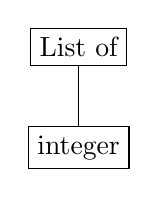
\begin{tikzpicture}
		\node[align=center, draw] (root)
		  {List of}
		;
		
    \draw (root) -- +(0, -1) node[draw, anchor=north](q) {integer};
		%  +(0,-1) 
\end{tikzpicture}
\begin{center}
(C) List of Temperatures
\end{center}

\end{center}
\caption{Weather Data Maps}
\label{data-maps-weather}
\end{figure}

Finding data sources can be a challenging task.
A component of my research plan is to publish best practices and techniques for finding, organizing, and exposing datasets.
The CORGIS collection already contains three dozen libraries, covering areas as diverse as international studies, nutrition, and social media platforms.
Some datasets were chosen because they were low-hanging fruit -- extensively documented, freely available, and well-supported. 
However, other datasets were driven by students' needs; in the two semesters that the course has been offered, two dozen new datasets have been created on demand.
The rapid turn-around time required has given new insight into the process of data mangling, although I am still exploring methods.
A massive part of my proposed work is to solidify and publish these techniques into a full paper.
